\documentclass[a4paper,
               11pt,
               parskip=half,
               headinclude,
               titlepage=false]{scrartcl}

%%%%%%%%%%%%%%%%%%%%%%%%%%%%%%%%%%%%%%%%
\newcommand{\metaauthor}{moPsy}
\newcommand{\metatitle}{DIV Assembly Guide}
\newcommand{\metarev}{1.1}
%%%%%%%%%%%%%%%%%%%%%%%%%%%%%%%%%%%%%%%%


\usepackage[utf8]{inputenc}

\usepackage[T1]{fontenc}        % Tries to use Postscript Type 1 Fonts for better rendering
\usepackage{lmodern}            % Provides the Latin Modern Font which offers more glyphs than the default Computer Modern
\usepackage[sfdefault]{carlito}
\usepackage[intlimits]{amsmath} % Provides all mathematical commands
\usepackage[protrusion=true,
            expansion,
            kerning=true,
            babel=true]{microtype}
\usepackage{fontawesome}

\usepackage[english]{babel}
\usepackage[english]{isodate}

\usepackage{eurosym}
\usepackage[shortlabels]{enumitem}

\usepackage{grffile}            % Allow you to include images (like graphicx). Usage: \includegraphics{path/to/file}

\usepackage[ugly]{units}        % Allows you to type units with correct spacing and font style. Usage: $\unit[100]{m}$ or $\unitfrac[100]{m}{s}$

\usepackage{xspace}             % Use \xpsace in macros to automatically insert space based on context. Usage: \newcommand{\es}{ESPResSo\xspace}
\usepackage[dvipsnames,table]{xcolor}             % Obviously colors. Usage: \color{red} Red text
\usepackage{booktabs}           % Nice rules for tables. Usage \begin{tabular}\toprule ... \midrule ... \bottomrule


%\usepackage[hang]{subfigure}  % unterteilte Abbildungen
\usepackage{setspace}          %fuer dem Zeilanabstand
\usepackage[hang,bf,footnotesize]{caption}   % bessere Bildunterschriften
\usepackage{wrapfig}

\usepackage{csquotes}


\usepackage[hyphens]{url}                % Lets you typeset urls. Usage: \url{http://...}
\usepackage[pdftex,colorlinks=true,linkcolor=black,citecolor=black,urlcolor=black]{hyperref}
\hypersetup{
  pdftitle    = {\metatitle},
  pdfsubject  = {Assembly Guide},
  pdfauthor   = {\metaauthor},
  pdfkeywords = {} ,
  pdfcreator  = {pdflatex},
  pdfproducer = {LaTeX with hyperref}
}
%%%%%%%%%%%%%%%%%%%%%%%%%%%%%%%%%%%%%%%%

\usepackage{pdfpages}

\usepackage{tabularx}


\usepackage[headsepline, footsepline]{scrlayer-scrpage}
\setlength{\headheight}{34pt} % logo height
\clearpairofpagestyles
\ohead{
\vfill%
\begin{tabular}{@{}l l@{}}

\includegraphics[height=2em]{moPsy_logo}\hspace*{-0.1cm}
\end{tabular}
}
\ihead{
\vfill%
{\huge DIV} \,v\metarev\, Assembly Guide%
}
\ofoot{Page \thepage}
\setkomafont{pageheadfoot}{\sffamily\footnotesize}
\setkomafont{pagination}{}
\pagestyle{scrheadings}


%\usepackage{background}

%\usepackage[section]{placeins} % keep figures in their section


\definecolor{level_easy}{rgb}{0.2, 0.6, 0.1}

\definecolor{row1}{rgb}{1.0, 1.0, 1.0}
\definecolor{row2}{rgb}{0.93, 0.93, 0.99}



\begin{document}


\begin{minipage}{12.5cm}
\setlength{\parskip}{\medskipamount}
\section*{Thank you for choosing a moPsy kit!}

\paragraph{tl;dr} Assembly is pretty straightforward. However, we strongly recommend soldering the transistors \emph{after} the LEDs to avoid Euclidean trouble.

This manual is meant to guide you through the assembly process.
We will point out common pitfalls when building this particular module.
Components are placed in an order that makes assembly as easy as possible.

This is an {\color{level_easy}easy} build, still there may be bugs in the instructions or something may not be communicated optimally.
If you happen to get stuck or something is not clear, feel free to send us a message and we will do our best to sort things out.

You can reach us at XXX.

Music is meant to be fun and enjoyment and we hope that you will enjoy building this module.
Please remember to take good care of yourself and get regular breaks whenever you start to feel exhausted. This is intended to be an afternoon stroll rather than a marathon.

\vspace{1em}
Enjoy building! \quad 
\includegraphics[height=0.8em]{peace_love_music}

\end{minipage}
\hspace{0.5cm}
\begin{minipage}{1.5cm}

\includegraphics[width=1.5cm]{div-frontpanel}
\end{minipage}

%\newpage
\subsection*{Resistors}

The resistors are color coded to identify their value. However, as these are sometimes hard to identify, we recommend using a multimeter to be sure.
Resistors do not have a polarity. Choosing a specific alignment is purely aesthetic.

\begin{tabularx}{\textwidth}{| r | l | X |}
\hline 
Qty & Value & Designator on PCB \\
\hline
14 & 
10k (brown, black, black, red, brown) & 
R1, R2, R3, R4, R6, R7, R8, R11, R12, R15, R18, R21, R24, R29 \\
\hline
12 &
2k2 (red, red, black, brown, brown) &
R13, R14, R16, R17, R19, R20, R22, R23, R25, R26, R27, R28 \\
\hline
3 &
1M (brown, black, black, yellow, brown) &
R5, R9, R10 \\
\hline  
\end{tabularx}


\subsection*{Diodes}

Diodes have a polarity! Please make sure that the black or white line on the diode matches with the line on the PCB.


\begin{tabularx}{\textwidth}{| r | l | X |}
\hline
Qty & Value & Designator on PCB \\
\hline
3 &
1N4148 (red) &
D3, D4, D5 \\
\hline
1 &
1N5817 (black) &
D17 \\
\hline
\end{tabularx}

\textbf{Please keep one of the legs of D17 for the ferrite beads!}


\subsection*{Ferrite Beads}

Use the leftover leg from D17 (above) to thread the ferrite bead and solder it like a resistor.

\begin{tabularx}{\textwidth}{| r |  X |}
\hline
Qty & Designator on PCB \\
\hline
1 &
FB1 \\
\hline
\end{tabularx}


\subsection*{IC and socket}

When placing the IC socket, please make sure that the notch is aligned with the notch on the PCB drawing. While the socket itself does not have an orientation, soldering it backwards will lead to confusion later.

Place the IC after the assembly of all components and take care of its orientation (notch or dot on the IC must match the notch on PCB and socket).

\begin{tabularx}{\textwidth}{| r | l | X |}
\hline
Qty & Value & Designator on PCB \\
\hline
1 &
4024 &
U1 \\
\hline
\end{tabularx}


\subsection*{Capacitors}

The ceramic capacitors (yellow) do not have a polarity and can be soldered in any orientation.
Have a look at \url{https://www.wikihow.com/Read-a-Capacitor} if you need help identifying capacitors.

\begin{tabularx}{\textwidth}{| r | l | X |}
\hline
Qty & Value & Designator on PCB \\
\hline
2 &
100n (Code 104) &
C1, C2 \\
\hline
\end{tabularx}


\subsection*{Electrolytic Capacitors}

Electrolytic capacitors \emph{do have a polarity} and are clearly marked with \texttt{+} or \texttt{-}. On the PCB, the white half of the marking is intended for the negative (\texttt{-}) side.

\begin{tabularx}{\textwidth}{| r | l | X |}
\hline
Qty & Value & Designator on PCB \\
\hline
1 &
10u (black) &
C3 \\
\hline
\end{tabularx}


\subsection*{Pin Headers}

Next up is the jumper for selecting the bus gate connection.

Solder the 2-pin header to J1.

When soldering, please make sure that the jumper sits straight on the PCB and does not lean out to the top. It may help to adjust while soldering the first pin. Be careful not to burn your fingers by not touching the part that you are currently soldering!


\subsection*{Mini Jacks}

Solder the eight mini jacks on J2 -- J9.

Please make sure they sit flush with the PCB, as they need to be aligned.
You can also put them in first, check with the front panel and then solder them.

Do not attach the front panel yet.


\subsection*{Power Connector}

Solder the power connector to J10.

Please make sure that the notch points to the edge of the PCB!

To make sure that the connector sits flush on the PCB, you can tag one pin first, then gently push the connector towards the PCBs and re-solder that pin. When you are happy with the alignment, solder the remaining pins (check again after the 2nd pin, after that, the position is fixed).


\subsection*{Front Panel}

Now it is time to assemble the front panel.
Just put it over the jacks and fix with the screws.

Please make sure that the orientation is correct, putting the clock input to the top (next to the Jumper) and the \enquote{64} output next to the power connector.


\subsection*{LEDs}

The LEDs are a bit tricky, but you have got help! 

If you turn the PCB over, there is a pending gauge to help with getting the lead lengths right: Place the LED into the hole so that the legs cover the lines on the PCB. 

Please make sure that the polarity is correct. The short leg (cathode) matches the \enquote{K} line, the long leg (anode) matches the \enquote{A} line.

When you are content with the LED alignment, bend the legs 90 degrees on the PCB edge.

Place the LED into its respective position on the PCB and its matching hole in the panel. When everything is aligned (short leg, i.e. cathode, to the square pad), solder the LED to the PCB.

We recommend fitting and soldering each LED individually.

\begin{tabularx}{\textwidth}{| r | l | X |}
\hline
Qty & Color & Designator on PCB \\
\hline
2 &
red &
D1, D6 \\
\hline
6 &
yellow &
D8, D10, D12, D14, D16, D19 \\
\hline
\end{tabularx}


\subsection*{Transistors}

Finally, solder the transistors. These have been left until now to make LED assembly easier.

With tweezers gently bend the center leg towards the round side of the package, then bend back until the legs are parallel again and match the footprint.

The transistors do not sit flush on the PCB, but hover a bit above it. Please do not apply too much force when pushing them in, as this may stress and break the package.
For nice alignment, it helps to solder the middle leg (base) first, then align the part and solder the other two legs.

\begin{tabularx}{\textwidth}{| r | l | X |}
\hline
Qty & Value & Designator on PCB \\
\hline
1 &
BC557 &
Q4 \\
\hline
9 &
BC547 &
Q1, Q2, Q3, Q5, Q6, Q7, Q8, Q9, Q10 \\
\hline
\end{tabularx}


\subsection*{IC}

Place the IC into its socket. It may help to carefully bend the legs on a flat surface.
Please make sure that the direction marks on the IC and the socket match (see also above).

\vspace{0.5cm}
\begin{center}
Enjoy your new module! \quad 
\includegraphics[height=0.8em]{peace_love_music}
\end{center}


\newpage

\section*{Silk Screen / Component Placement}
\begin{center}
\begin{minipage}{.35\linewidth}
  
\includegraphics[width=\linewidth]{div-F_Silkscreen}
\end{minipage}
\hspace{.1\linewidth}
\begin{minipage}{.35\linewidth}
  \includegraphics[width=\linewidth]{div-B_Silkscreen}
\end{minipage}
\end{center}

\newpage



\section*{Assembly Variants}

If you just want to build the kit, please ignore this section.

There are two ways in which you may want to deviate from the build instructions, which are described below.
Please note that we do not provide the necessary parts to implement these changes with our kits. 

\subsection*{DIV Glow}

The \emph{DIV glow} variant uses SMD LEDs and transparent jacks instead of separate panel LEDs. The changes are:
\begin{itemize}[noitemsep]
 \item Populate D2, D7, D9, D11, D13, D15, D18, D20 with 0604in-sized LEDs. We recommend using extra bright LEDs (around \unit[200]{mcd}), especially if you do not want to tweak the LED resistors. 
 \item DO NOT populate D1, D6, D8, D10, D12, D14, D16, D19.
 \item Adjust the LED resistors accordingly (see below).
 \item We recommend using the \emph{DIV glow} panel.
\end{itemize}

\subsection*{LED resistors}

To tweak the LED brightness or if you are not using extra bright LEDs (around \unit[200]{mcd}), you can adjust the LED resistors accordingly.

From top to bottom on the panel, these are: R1, R6, R12, R15, R18, R21, R24, R29.

Please note that the power ratings change with these LEDs and the module might source much more current than expected.

We strongly recommend sticking to extra bright LEDs. However, lowering the LED resistors to \unit[4.7]{k} might improve your experience while staying within an acceptable power consumption.

\subsection*{No Bus Reset}

You can leave out the Bus reset feature. The components involved are so cheap that we only recommend this step if there is a real reason. (Please let us know when this happens!)

To skip the bus access, do not populate these components: R2, R9, D5, Q3, J1

\end{document}
